%%%%%%%%%%%%%%%%%%%%%%%%%%%%%%%%%%%%%%%%%
% Arsclassica Article
% LaTeX Template
% Version 1.1 (10/6/14)
%
% This template has been downloaded from:
% http://www.LaTeXTemplates.com
%
% Original author:
% Lorenzo Pantieri (http://www.lorenzopantieri.net) with extensive modifications by:
% Vel (vel@latextemplates.com)
%
% License:
% CC BY-NC-SA 3.0 (http://creativecommons.org/licenses/by-nc-sa/3.0/)
%
%%%%%%%%%%%%%%%%%%%%%%%%%%%%%%%%%%%%%%%%%

%----------------------------------------------------------------------------------------
%	PACKAGES AND OTHER DOCUMENT CONFIGURATIONS
%----------------------------------------------------------------------------------------

\documentclass[
10pt, % Main document font size
a4paper, % Paper type, use 'letterpaper' for US Letter paper
oneside, % One page layout (no page indentation)
%twoside, % Two page layout (page indentation for binding and different headers)
headinclude,footinclude, % Extra spacing for the header and footer
BCOR5mm, % Binding correction
]{scrartcl}

%----------------------------------------------------------------------------------------

\usepackage{listings} % Required for inserting code snippets
\usepackage[usenames,dvipsnames]{xcolor} % Required for specifying custom colors and referring to colors by name
\usepackage[titletoc,title]{appendix}
\usepackage{ amssymb }
\usepackage{hyperref}

\definecolor{DarkGreen}{rgb}{0.0,0.4,0.0} % Comment color
\definecolor{highlight}{RGB}{255,251,204} % Code highlight color

\lstdefinestyle{Style1}{ % Define a style for your code snippet, multiple definitions can be made if, for example, you wish to insert multiple code snippets using different programming languages into one document
language=Fortran, % Detects keywords, comments, strings, functions, etc for the language specified
backgroundcolor=\color{highlight}, % Set the background color for the snippet - useful for highlighting
basicstyle=\footnotesize\ttfamily, % The default font size and style of the code
breakatwhitespace=false, % If true, only allows line breaks at white space
breaklines=true, % Automatic line breaking (prevents code from protruding outside the box)
captionpos=b, % Sets the caption position: b for bottom; t for top
commentstyle=\usefont{T1}{pcr}{m}{sl}\color{DarkGreen}, % Style of comments within the code - dark green courier font
deletekeywords={}, % If you want to delete any keywords from the current language separate them by commas
%escapeinside={\%}, % This allows you to escape to LaTeX using the character in the bracket
firstnumber=1, % Line numbers begin at line 1
frame=single, % Frame around the code box, value can be: none, leftline, topline, bottomline, lines, single, shadowbox
frameround=tttt, % Rounds the corners of the frame for the top left, top right, bottom left and bottom right positions
keywordstyle=\color{Blue}\bf, % Functions are bold and blue
morekeywords={}, % Add any functions no included by default here separated by commas
numbers=left, % Location of line numbers, can take the values of: none, left, right
numbersep=10pt, % Distance of line numbers from the code box
numberstyle=\tiny\color{Gray}, % Style used for line numbers
rulecolor=\color{black}, % Frame border color
showstringspaces=false, % Don't put marks in string spaces
showtabs=false, % Display tabs in the code as lines
stepnumber=5, % The step distance between line numbers, i.e. how often will lines be numbered
stringstyle=\color{Purple}, % Strings are purple
tabsize=2, % Number of spaces per tab in the code
}

%%%%%%%%%%%%%%%%%%%%%%%%%%%%%%%%%%%%%%%%%
% Arsclassica Article
% Structure Specification File
%
% This file has been downloaded from:
% http://www.LaTeXTemplates.com
%
% Original author:
% Lorenzo Pantieri (http://www.lorenzopantieri.net) with extensive modifications by:
% Vel (vel@latextemplates.com)
%
% License:
% CC BY-NC-SA 3.0 (http://creativecommons.org/licenses/by-nc-sa/3.0/)
%
%%%%%%%%%%%%%%%%%%%%%%%%%%%%%%%%%%%%%%%%%

%----------------------------------------------------------------------------------------
%	REQUIRED PACKAGES
%----------------------------------------------------------------------------------------

\usepackage[
nochapters, % Turn off chapters since this is an article        
beramono, % Use the Bera Mono font for monospaced text (\texttt)
eulermath,% Use the Euler font for mathematics
pdfspacing, % Makes use of pdftex’ letter spacing capabilities via the microtype package
dottedtoc % Dotted lines leading to the page numbers in the table of contents
]{classicthesis} % The layout is based on the Classic Thesis style

\usepackage{arsclassica} % Modifies the Classic Thesis package

\usepackage[T1]{fontenc} % Use 8-bit encoding that has 256 glyphs

\usepackage[utf8]{inputenc} % Required for including letters with accents

\usepackage{graphicx} % Required for including images
\graphicspath{{Figures/}} % Set the default folder for images

\usepackage{enumitem} % Required for manipulating the whitespace between and within lists

\usepackage{lipsum} % Used for inserting dummy 'Lorem ipsum' text into the template

\usepackage{subfig} % Required for creating figures with multiple parts (subfigures)

\usepackage{amsmath,amssymb,amsthm} % For including math equations, theorems, symbols, etc

\usepackage{varioref} % More descriptive referencing

%----------------------------------------------------------------------------------------
%	THEOREM STYLES
%---------------------------------------------------------------------------------------

\theoremstyle{definition} % Define theorem styles here based on the definition style (used for definitions and examples)
\newtheorem{definition}{Definition}

\theoremstyle{plain} % Define theorem styles here based on the plain style (used for theorems, lemmas, propositions)
\newtheorem{theorem}{Theorem}

\theoremstyle{remark} % Define theorem styles here based on the remark style (used for remarks and notes)

%----------------------------------------------------------------------------------------
%	HYPERLINKS
%---------------------------------------------------------------------------------------

\hypersetup{
%draft, % Uncomment to remove all links (useful for printing in black and white)
colorlinks=true, breaklinks=true, bookmarks=true,bookmarksnumbered,
urlcolor=webbrown, linkcolor=RoyalBlue, citecolor=webgreen, % Link colors
pdftitle={}, % PDF title
pdfauthor={\textcopyright}, % PDF Author
pdfsubject={}, % PDF Subject
pdfkeywords={}, % PDF Keywords
pdfcreator={pdfLaTeX}, % PDF Creator
pdfproducer={LaTeX with hyperref and ClassicThesis} % PDF producer
}
 % Include the structure.tex file which specified the document structure and layout

\hyphenation{Fortran hy-phen-ation} % Specify custom hyphenation points in words with dashes where you would like hyphenation to occur, or alternatively, don't put any dashes in a word to stop hyphenation altogether

\setcounter{secnumdepth}{5}


% Create a command to cleanly insert a snippet with the style above anywhere in the document
\newcommand{\insertcode}[2]{\begin{itemize}\item[]\lstinputlisting[caption=#2,label=#1,style=Style1]{#1}\end{itemize}} % The first argument is the script location/filename and the second is a caption for the listing

%----------------------------------------------------------------------------------------
%	TITLE AND AUTHOR(S)
%----------------------------------------------------------------------------------------

\title{\normalfont\spacedallcaps{Molecular dynamics simulation of Argon}} % The article title

\author{\spacedlowsmallcaps{Alexander Cronheim\textsuperscript{1} \& Aboubakr El Mahdaoui\textsuperscript{1}}} % The article author(s) - author affiliations need to be specified in the AUTHOR AFFILIATIONS block

\date{} % An optional date to appear under the author(s)

%----------------------------------------------------------------------------------------

\begin{document}

%----------------------------------------------------------------------------------------
%	HEADERS
%----------------------------------------------------------------------------------------

\renewcommand{\sectionmark}[1]{\markright{\spacedlowsmallcaps{#1}}} % The header for all pages (oneside) or for even pages (twoside)
%\renewcommand{\subsectionmark}[1]{\markright{\thesubsection~#1}} % Uncomment when using the twoside option - this modifies the header on odd pages
\lehead{\mbox{\llap{\small\thepage\kern1em\color{halfgray} \vline}\color{halfgray}\hspace{0.5em}\rightmark\hfil}} % The header style

\pagestyle{scrheadings} % Enable the headers specified in this block

%----------------------------------------------------------------------------------------
%	TABLE OF CONTENTS & LISTS OF FIGURES AND TABLES
%----------------------------------------------------------------------------------------

\maketitle % Print the title/author/date block

\setcounter{tocdepth}{2} % Set the depth of the table of contents to show sections and subsections only

\tableofcontents % Print the table of contents

\listoffigures % Print the list of figures

\listoftables % Print the list of tables

{\let\thefootnote\relax\footnotetext{\textsuperscript{1} \textit{Faculty of Applied Physics, University of Techonology, Delft, the Netherlands}}}

\newpage % Start the article content on the second page, remove this if you have a longer abstract that goes onto the second page

%----------------------------------------------------------------------------------------
%	ABSTRACT
%----------------------------------------------------------------------------------------

\section*{Abstract} % This section will not appear in the table of contents due to the star (\section*)

The motion of a collection of 864 particles has been simulated using Molecular Dynamics techniques to compute values for pressure, specific heat and the static pair correlation function in reduced units. The computed properties were compared with experimental results for the properties of argon. The simulation was done with a Lennard-Jones pair-potential and the system was allowed to reach equilibrium. The computed results are in good agreement with the known properties of argon.

%\lipsum[1] % Dummy text

%----------------------------------------------------------------------------------------
%	AUTHOR AFFILIATIONS
%----------------------------------------------------------------------------------------

%{\let\thefootnote\relax\footnotetext{* \textit{Faculty of Applied Physics, University of Techonology, Delft, the Netherlands}}}


%----------------------------------------------------------------------------------------

\newpage % Start the article content on the second page, remove this if you have a longer abstract that goes onto the second page

%----------------------------------------------------------------------------------------
%	INTRODUCTION
%----------------------------------------------------------------------------------------

\section{Introduction}

Molecular dynamics is a method to simulate a many-particle system by numerically solving Newton's classical equations of motion for all particles for a period of time. The main limitations are the fact that simulations are only  realizable for small systems  and times compared to experimental systems in general. Furthermore, the systems to be simulated can only be classical in the usual molecular dynamics approach. 

In this report we discuss the results of simulations for a system of argon gas with 864 particles. Molecular dynamics simulations of argon are reported to be in good agreement with experimental results\cite{Verlet:1967md}. The particles are placed in a FCC lattice, considering the fact that the ground state configuration is a FCC lattice for argon. A Lennard-Jones Potential is implemented for the calculation of the force between the particles where a pair potential is assumed. The initial velocities of the particles are randomly generated for each velocity component while obeying a Maxwell-Boltzmann distribution for all particles. 

After initialization the system's equations of motion are solved numerically after each time step using Verlet's algorithm. The system is allowed to relax to it's equilibrium using a thermostat to rescale the velocities and enforce energy conservation. After the equilibrium has been reached, the simulation continues and collects results for calculating the time average of different properties of the system. The virial's theorem allows the calculation of the pressure, specific heat is evaluated using a formula derived by Lebowitz using the fluctuations of the kinetic energy\cite{Duane:1985lz}.

 
\newpage
%----------------------------------------------------------------------------------------
%	THEORY
%----------------------------------------------------------------------------------------

\section{Theory}

\subsection{Lennard Jones Potential}

The Lennard Jones pair potential describes a potential between atoms and models a repulsive term and an attractive term as follows:

$$ V_{LJ} =  4 \epsilon \left [ \left (\frac{\sigma}{r} \right )^{12} - \left ( \frac{\sigma}{r} \right )^6 \right ] $$

For argon this has been working quite well as a good mathematical model for all three phases\cite{Rahman}. 
 

\subsection{Virial Theorem}

\subsection{Specific Heat}

The specific heat at constant volume $C_V$  is defined as:
$$ C_V = \left ( \frac{\delta E}{\delta T} \right )_V $$

\noindent
In molecular dynamics simulations, a quantity that can be calculated is the ensemble average of the total energy $\langle E\rangle_{NVT}$:

$$ \langle E\rangle_{NVT} = \frac{ \sum_X e^{-\beta \mathcal{H}(X)} \mathcal{H}(X)}{ \sum_X e^{-\beta \mathcal{H}(X)}} = - \frac{\delta ln(Z)}{\delta \beta} $$

\noindent
Using the ensemble average for the total energy, the formula for the specific heat can be rewritten as a function of the fluctuations in the total energy:

\begin{align}
C_V &= \frac{1}{k_B T^2} \frac{\delta^2 ln(Z)}{\delta \beta^2} \\
&= \frac{1}{k_B T^2} \left ( \langle E^2\rangle_{NVT} - \langle E\rangle^2_{NVT} \right )
\end{align}

\noindent
This is still difficult to use in a program simulating a system in the microcanonical ensemble as the total energy is kept fixed, but following the derivation by Lebowitz\cite{Duane:1985lz} this can be related to the fluctuation in kinetic energy:

$$ \frac{\langle\delta K^2\rangle}{\langle K\rangle^2} = \frac{2}{3N} \left ( 1 - \frac{3N}{2C_V} \right ) $$



\subsection{Pair correlation function}

The static pair correlation function in the canonical ensemble can be expressed as:

$$ g(\mathbf{r,r'}) = V^2 \frac{1}{N!h^{3N}Z} \int_V d^3r_3....d^3r_N e^{-\beta V_N(\mathbf{r,r',r_3.....r_N})} $$

\noindent
If the system is homogeneous and has a large number of particles $N$, it can also be written as a function of the difference $\mathbf{\Delta r} = \mathbf{r} - \mathbf{r'}$:

$$ g(\mathbf{\Delta r}) = \frac{V}{N(N-1)}  \left \langle \int d^3r' \sum_{i,j i \neq j}^N \delta(\mathbf{r}-\mathbf{r}_i) \delta(\mathbf{r'} + \Delta\mathbf{r} - \mathbf{r}_j) \right \rangle $$

\newpage
%----------------------------------------------------------------------------------------
%	METHODS
%----------------------------------------------------------------------------------------

\section{Methods for Simulation}

\subsection{Initialization}

The system is initialized by creating an fcc lattice structure and assigning each position of the particles to the lattice points. This is done for 864 particles but can in principle be easily implemented for a number of particles $N$ that can be written as $4M^3$ with $M$ an integer and representing the number of fcc cells in one dimension.

\insertcode{"Scripts/initialization_snippet_1.f90"}{Constructing the fcc lattice} % The first argument is the script location/filename and the second is a caption for the listing

Above can you see the code with $i$, $j$ and $k$ for the $x$, $y$ and $z$ component and a function fcc\_cell is called that takes an argument $l$ to add the relative position of each particle in a particular cell.


\subsubsection{Velocity Distribution}

The particles are then assigned an initial velocity that is randomly distributed but the distribution in each direction obeys a Maxwell-Boltzmann distribution:
$$ f(v_i) = \sqrt{\frac{m}{2\pi k_B T}} e^{\frac{-mv_i^2}{2k_BT}} $$

\insertcode{"Scripts/initialization_snippet_2.f90"}{Generating initial velocities} % The first argument is the script location/filename and the second is a caption for the listing

\insertcode{"Scripts/initialization_snippet_3.f90"}{Removing the center of mass degree of freedom} % The first argument is the script location/filename and the second is a caption for the listing

\paragraph{Box Muller Algorithm}


\subsection{Dynamics}

\subsubsection{Boundary Conditions}
As the system to be simulated is very small compared to real experimental systems, boundaries would probably have a larger effect in the simulation. To counter this periodic boundary conditions are used and this is implemented by copying the system in all directions creating a large box of 9 identical smaller boxes with the box in the middle as our box of interest. As we calculate the forces the Lennard Jones pair potential is calculated for all the particles inside the box and also all the other 8 copies that are closer than a predefined cut off distance. 

\insertcode{"Scripts/boundary_conditions_snippet_1.f90"}{Creating periodic boundary conditions} % The first argument is the script location/filename and the second is a caption for the listing





\subsubsection{Lennard Jones Potential}

 
\subsubsection{Force Calculation}

\paragraph{Leap Frog/Verlet Algorithm}

\subsubsection{Pressure Calculation}

\paragraph{Virial Theorem}

\subsubsection{Thermostat}

\subsection{Information Processing}

\subsubsection{Specific Heat}

The implementation in our simulation is inside the algorithm for the dynamics of the particles. For each time step the new velocities are calculated, the kinetic energy is also calculated and the relevant sums of the kinetic energy are updated in a subroutine "calc\_specific\_heat":

\insertcode{"Scripts/specific_heat_snippet_1.f90"}{Updating the relevant sums of the kinetic energy} % The first argument is the script location/filename and the second is a caption for the listing

\noindent
As discussed earlier, the specific heat is related to the fluctuations in kinetic energy using a formula derived by Lebowitz\cite{Duane:1985lz}:

$$ \frac{\langle\delta K^2\rangle}{\langle K\rangle^2} = \frac{2}{3N} \left ( 1 - \frac{3N}{2C_V} \right ) $$

\noindent
Rewriting this to get an expression for the specific heat:

\begin{align}
C_V &= \left (\frac{2}{3N} - \frac{\langle\delta K^2\rangle}{\langle K\rangle^2}\right)^{-1} \\
&= \left (\frac{2}{3N} - \frac{\langle K^2 \rangle - \langle K \rangle^2}{\langle K\rangle^2} \right )^{-1} 
\end{align}


\noindent
Using the time average instead of the ensemble average, the averages can be expressed as a sum over all time steps $n_t$ divided by the time steps:
$$ \langle K^2 \rangle  = \frac{\sum_{i=1}^{n_t} K(i)^2}{n_t} $$
$$ \langle K \rangle^2  = \left ( \frac{\sum_{i=1}^{n_t} K(i)  }{n_t} \right)^2 $$

\noindent
Now the specific heat can be calculated as:
\begin{align}
C_V &= \left (\frac{2}{3N} - \frac{\langle K^2 \rangle - \langle K \rangle^2}{\langle K\rangle^2} \right )^{-1} \\
&= \left ( \frac{2}{3N} - \frac{\sum_{i=1}^{n_t} K(i)^2*n_t - \left (\sum_{i=1}^{n_t} K(i) \right )^2 }{\left (\sum_{i=1}^{n_t} K(i) \right )^2 } \right )^{-1}
\end{align}

This is implemented in our code within the same subroutine "calc\_specific\_heat" after an if statement is enabled at the end of the simulation:
\insertcode{"Scripts/specific_heat_snippet_2.f90"}{Calculating the specific heat} % The first argument is the script location/filename and the second is a caption for the listing


\subsubsection{Pair Correlation Function}

The pair correlation function can be evaluated in molecular dynamics systems  if a histogram is recorded of the number of pairs of particles $n(r)$ for each distance $r$:

$$ g(r) = \frac{2V}{N(N-1)} \left [ \frac{\langle n(r) \rangle }{ 4 \pi r^2 \Delta r} \right ] $$

\noindent
In our simulation a number of intervals $n_i$ is defined which together with the length in each direction $L$ sets the small $\Delta r$:

$$ \Delta r  = \frac{L}{n_i} $$

\noindent
Again a time average is used and the average number of pairs $\langle n(r) \rangle $ is calculated as a sum of all the pair occurences $N(r,t)$ in a time step $t$ and in a distance $r$ over all time steps $n_t$:
$$ \langle n(r) \rangle = \frac{\sum_t^{n_t} N(r,t)}{n_t} $$

\noindent
For a large enough number of intervals the distance $r$ can be approximated by $i\Delta r$ with $i$ the index of the corresponding interval. The number of pair occurences $N(r,t)$ in a time step $t$ and in a distance $r$ can be expressed now as function of the interval you are in $N(i,t)$. This way we are able to count all pair occurences in our program and calculate the pair correlation function:

\begin{align}
g(r) &\approx \frac{2V}{N(N-1)} \left [ \frac{\langle n(r) \rangle }{ 4 \pi r^2 \Delta r} \right ] \\
&= \frac{2L^3}{N(N-1)} \left [ \frac{\sum_t^{n_t} N(i,t)}{n_t 4 \pi i^2 \Delta r^2 \Delta r} \right ] \\
&= \frac{2L^3}{N(N-1)} \frac{\sum_t^{n_t} N(i,t)}{n_t 4 \pi i^2} \frac{n_i^3}{L^3} \\
&= \frac{2}{N(N-1)} \frac{n_i^3}{n_t 4 \pi} \frac{\sum_t^{n_t} N(i,t)}{i^2}
\end{align}

\noindent
This is implemented in the code as follows. For each interval $i$ the number of pair occurences in that interval is registered in a particular time interval. This is done while evaluating the forces of the particles:
\insertcode{"Scripts/pair_correlation_snippet_1.f90"}{Updating the histogram for each interval} % The first argument is the script location/filename and the second is a caption for the listing

\noindent
As the final time step is done and the routine for the dynamics is finished, the sum for each interval is passed to a routine for calculating the pair correlation function that is called at the end:
\insertcode{"Scripts/pair_correlation_snippet_2.f90"}{Factors are needed to prevent overflow errors} % The first argument is the script location/filename and the second is a caption for the listing








\newpage
%----------------------------------------------------------------------------------------
%	RESULTS AND DISCUSSION
%----------------------------------------------------------------------------------------

\section{Results and Discussion}

\subsection{Pressure \& Temperature}
In this section the results for pressure and temperature is compared with the values of table ~\vref{tab:label} for molecular dynamics simulation of a Lennard Jones liquid in \cite{Thijssen:2013cp}

\begin{table}[hbt]
\caption{Molecular dynamics data for thermodynamic quantities of the Lennard–Jones liquid.}
\centering
\begin{tabular}{lllll}
\toprule
\toprule
%\multicolumn{2}{c}{Name} \\
%\cmidrule(r){1-2}
$\rho(1/\sigma^3)$ & $T_0(\epsilon/k_B)$ & $T$ & $\beta P/\rho$ & $U(\epsilon)$ \\
\midrule
$0.88$ & $1.0$ & $0.990$ & $2.98$ & $-5.704$ \\
$0.8$ & $1.0$ & $1.010$ & $1.31$ & $-5.271$ \\
$0.7$ & $1.0$ & $1.014$ & $1.06$ & $-4.662$ \\
\bottomrule
\bottomrule
\end{tabular}
\label{tab:label}
\end{table}


%------------------------------------------------

\subsection{Specific Heat}




Some text with a citation \cite{Verlet:1967md}
The other citation \cite{Glosser:2015iccp} and another\cite{Thijssen:2013cp}


\subsection{Pair Correlation function}

The pair correlation function is plotted for $\rho = 0.88$ and different values of $T$ in Figure~\vref{fig:correlation}. It can be seen that the correlation function tends to 1 as expected in all cases. Furthermore, the repulsive term of the Lennard Jones potential prevents particles being close together as can be seen in the pair correlation. For $\rho = 0.88$, there is also a phase transition taking place between the temperatures $T=0.8$ and $T=0.6$ where solid argon shows a different pair correlation function with respect to liquid argon. For liquid argon the pair correlation function is simply oscillating indicating what the average distance is between  particles. As you move further away from a particular particle, the fluctuations in the average distances cause the peaks to broaden as well as the peaks to be lower for longer distances in the liquid argon. The solid argon shows peaks where the first, second etc. neighbors are in a lattice structure and shows a more complex function, but the oscillations tend to be more persistent even along longer distances compared to liquid argon as can be expected because of the periodic lattice structure. The results presented show good agreement with other experiments\cite{Thijssen:2013cp}. 

%The pair correlation function is plotted for $\rho = 0.88$ and $T=0.6$~\vref{fig:gallery}. It can be seen that this tends to 1 and is typical for solid argon. % The \vref command specifies the location of the reference

\begin{figure}[tb]
\centering
\subfloat[Pair correlation function of Argon($\rho = 0.88$, $T=0.2$) ]{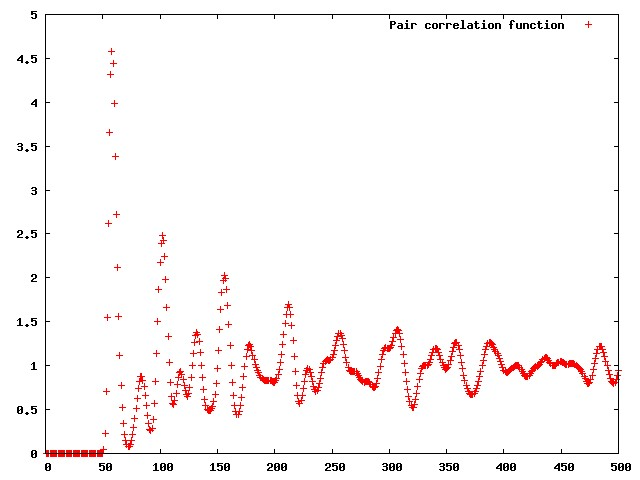
\includegraphics[width=.45\columnwidth]{histogramrho088T02}} \quad
\subfloat[Pair correlation function of Argon($\rho = 0.88$, $T=0.4$) ]{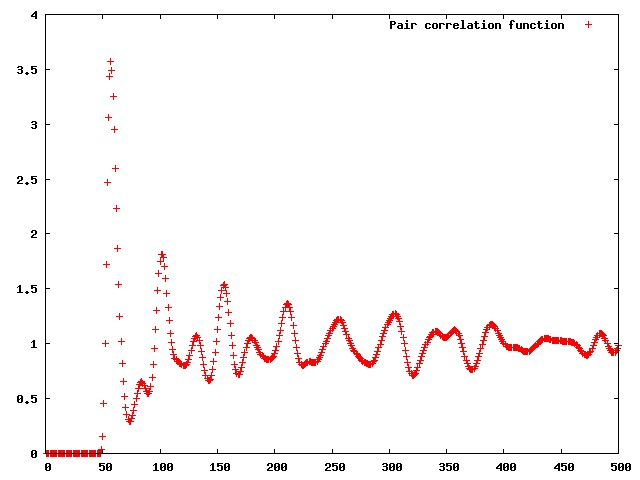
\includegraphics[width=.45\columnwidth]{histogramrho088T04}\label{fig:ipsum}} \\
\subfloat[Pair correlation function of Argon($\rho = 0.88$, $T=0.6$) ]{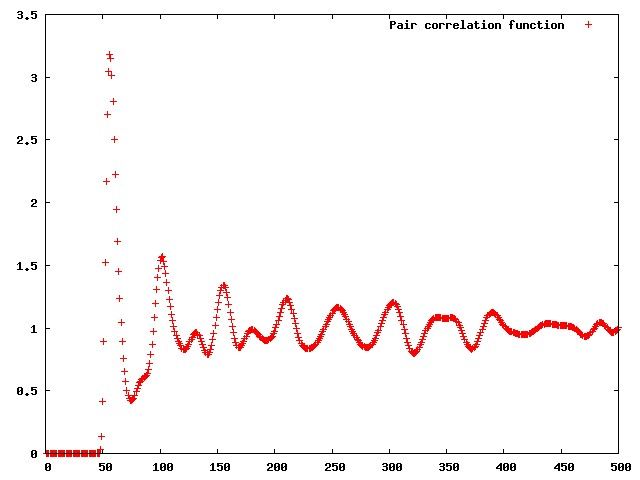
\includegraphics[width=.45\columnwidth]{histogramrho088T06}} \quad
\subfloat[Pair correlation function of Argon($\rho = 0.88$, $T=0.8$) ]{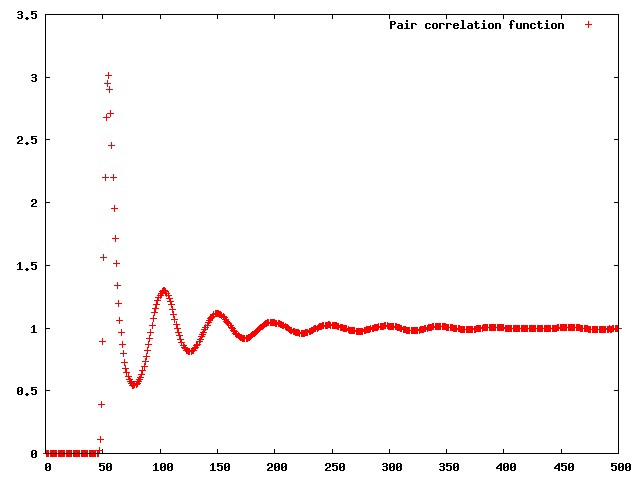
\includegraphics[width=.45\columnwidth]{histogramrho088T08}}
\caption[Pair correlation function of Argon($\rho = 0.88$, $T=0.6$) ]{Phase transition shown in pair correlation} % The text in the square bracket is the caption for the list of figures while the text in the curly brackets is the figure caption
\label{fig:correlation}
\end{figure}

%\begin{figure}[tb]
%\centering 
%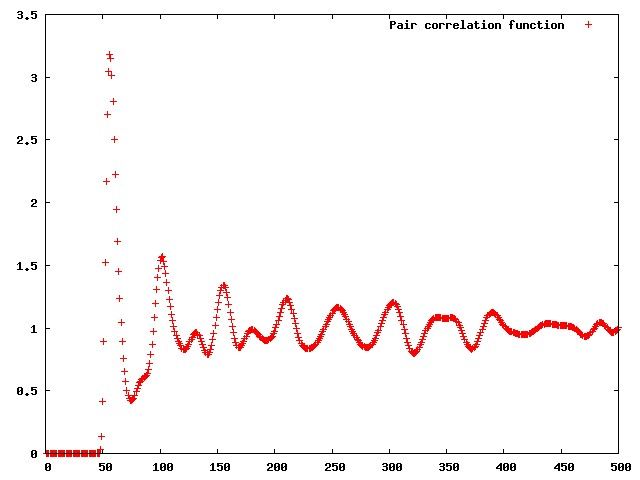
\includegraphics[width=0.5\columnwidth]{histogramrho088T06} 
%\caption[Pair correlation function of solid Argon($\rho = 0.88$, $T=0.6$) ]{Pair correlation function of solid Argon ($\rho = 0.88$, $T=0.6$)} % The text in the square bracket is the caption for the list of figures while the text in the curly brackets is the figure caption
%\label{fig:gallery} 
%\end{figure}



%------------------------------------------------


%----------------------------------------------------------------------------------------
%	BIBLIOGRAPHY
%----------------------------------------------------------------------------------------

\newpage

\renewcommand{\refname}{\spacedlowsmallcaps{References}} % For modifying the bibliography heading

\bibliographystyle{unsrt}

\bibliography{sample.bib} % The file containing the bibliography

%----------------------------------------------------------------------------------------


%----------------------------------------------------------------------------------------
%	APPENDIX
%----------------------------------------------------------------------------------------

\newpage

\begin{appendices}

\section{Main Fortran source code}

%----------------------------------------------------------------------------------------

\insertcode{"../argon_box.f90"}{argon\_box.f90} % The first argument is the script location/filename and the second is a caption for the listing

%----------------------------------------------------------------------------------------

\newpage


\section{Fortran source code for setting the initial conditions}

%----------------------------------------------------------------------------------------

\insertcode{"../argon_box_init.f90"}{argon\_box\_init.f90} % The first argument is the script location/filename and the second is a caption for the listing

%----------------------------------------------------------------------------------------

\newpage


\section{Fortran source code for the dynamics of the system}

%----------------------------------------------------------------------------------------

\insertcode{"../argon_box_dynamics.f90"}{argon\_box\_dynamics.f90} % The first argument is the script location/filename and the second is a caption for the listing

%----------------------------------------------------------------------------------------

\newpage


\section{Fortran source code for output of results}

%----------------------------------------------------------------------------------------

\insertcode{"../argon_box_results.f90"}{argon\_box\_results.f90} % The first argument is the script location/filename and the second is a caption for the listing

%----------------------------------------------------------------------------------------

\newpage

\end{appendices}

\end{document}



















